%========= File containing the main LaTex document ========%
%                                                          %
% Copyright (C) ISI - All Rights Reserved                  %
% Proprietary                                              %
% Written by Med Hossam <med.hossam@gmail.com>, April 2016 %
%                                                          %
% @author: HEDHILI Med Houssemeddine                       %
% @linkedin: http://tn.linkedin.com/in/medhossam           %
%==========================================================%

%\documentclass[pfe]{./tpl/isipfe}
\documentclass[]{./tpl/isipfe}
\graphicspath{{./img/}}

%\usepackage{hyperref}


%=========== File containing some new commands ============%
%                                                          %
% Copyright (C) ISI - All Rights Reserved                  %
% Proprietary                                              %
% Written by Med Hossam <med.hossam@gmail.com>, April 2016 %
%                                                          %
% @author: HEDHILI Med Houssemeddine                       %
% @linkedin: http://tn.linkedin.com/in/medhossam           %
%==========================================================%

\newenvironment{changemargin}[2]{%
\begin{list}{}{%
\setlength{\leftmargin}{#1}%
\setlength{\rightmargin}{#2}%
}%
\item[]}
{\end{list}}

\makeatletter

%================= front cover variables =================%

\newcommand{\secondAuthor}[1]{\gdef\@secondAuthor{#1}}%
\newcommand{\@secondAuthor}{\@latex@warning@no@line{No \noexpand\secondAuthor given}}

\newcommand{\diplomaName}[1]{\gdef\@diplomaName{#1}}%
\newcommand{\@diplomaName}{\@latex@warning@no@line{No \noexpand\diplomaName given}}

\newcommand{\speciality}[1]{\gdef\@speciality{#1}}%
\newcommand{\@speciality}{\@latex@warning@no@line{No \noexpand\speciality given}}

\newcommand{\proFramerName}[1]{\gdef\@proFramerName{#1}}%
\newcommand{\@proFramerName}{\@latex@warning@no@line{No \noexpand\proFramerName given}}

\newcommand{\proFramerSpeciality}[1]{\gdef\@proFramerSpeciality{#1}}%
\newcommand{\@proFramerSpeciality}{\@latex@warning@no@line{No \noexpand\proFramerSpeciality given}}

\newcommand{\academicFramerName}[1]{\gdef\@academicFramerName{#1}}%
\newcommand{\@academicFramerName}{\@latex@warning@no@line{No \noexpand\academicFramerName given}}

\newcommand{\academicFramerSpeciality}[1]{\gdef\@academicFramerSpeciality{#1}}%
\newcommand{\@academicFramerSpeciality}{\@latex@warning@no@line{No \noexpand\academicFramerSpeciality given}}

\newcommand{\collegeYear}[1]{\gdef\@collegeYear{#1}}%
\newcommand{\@collegeYear}{\@latex@warning@no@line{No \noexpand\collegeYear given}}

\newcommand{\companyName}[1]{\gdef\@companyName{#1}}%
\newcommand{\@companyName}{\@latex@warning@no@line{No \noexpand\companyName given}}

%================== Signatures variables ==================%

\newcommand{\proSignSentence}[1]{\gdef\@proSignSentence{#1}}%
\newcommand{\@proSignSentence}{\@latex@warning@no@line{No \noexpand\proSignSentence given}}

\newcommand{\academicSignSentence}[1]{\gdef\@academicSignSentence{#1}}%
\newcommand{\@academicSignSentence}{\@latex@warning@no@line{No \noexpand\academicSignSentence given}}

%================== Backcover variables ==================%

\newcommand{\arabicAbstract}[1]{\gdef\@arabicAbstract{#1}}%
\newcommand{\@arabicAbstract}{\@latex@warning@no@line{No \noexpand\arabicAbstract given}}

\newcommand{\arabicAbstractKeywords}[1]{\gdef\@arabicAbstractKeywords{#1}}%
\newcommand{\@arabicAbstractKeywords}{\@latex@warning@no@line{No \noexpand\arabicAbstractKeywords given}}

\newcommand{\frenchAbstract}[1]{\gdef\@frenchAbstract{#1}}%
\newcommand{\@frenchAbstract}{\@latex@warning@no@line{No \noexpand\frenchAbstract given}}

\newcommand{\frenchAbstractKeywords}[1]{\gdef\@frenchAbstractKeywords{#1}}%
\newcommand{\@frenchAbstractKeywords}{\@latex@warning@no@line{No \noexpand\frenchAbstractKeywords given}}

\newcommand{\englishAbstract}[1]{\gdef\@englishAbstract{#1}}%
\newcommand{\@englishAbstract}{\@latex@warning@no@line{No \noexpand\englishAbstract given}}

\newcommand{\englishAbstractKeywords}[1]{\gdef\@englishAbstractKeywords{#1}}%
\newcommand{\@englishAbstractKeywords}{\@latex@warning@no@line{No \noexpand\englishAbstractKeywords given}}

\newcommand{\companyEmail}[1]{\gdef\@companyEmail{#1}}%
\newcommand{\@companyEmail}{\@latex@warning@no@line{No \noexpand\companyEmail given}}

\newcommand{\companyTel}[1]{\gdef\@companyTel{#1}}%
\newcommand{\@companyTel}{\@latex@warning@no@line{No \noexpand\companyTel given}}

\newcommand{\companyFax}[1]{\gdef\@companyFax{#1}}%
\newcommand{\@companyFax}{\@latex@warning@no@line{No \noexpand\companyFax given}}

\newcommand{\companyAddressFR}[1]{\gdef\@companyAddressFR{#1}}%
\newcommand{\@companyAddressFR}{\@latex@warning@no@line{No \noexpand\companyAddressFR given}}

\newcommand{\companyAddressAR}[1]{\gdef\@companyAddressAR{#1}}%
\newcommand{\@companyAddressAR}{\@latex@warning@no@line{No \noexpand\companyAddressAR given}}

%============= cmd for inserting blank page =============%
\newcommand\blankpage{%
    \null
    \thispagestyle{empty}%
    \addtocounter{page}{-1}%
    \newpage}

%================ document main language ================%
%\selectlanguage{english}
\selectlanguage{french}

%================== required packages ===================%

\usepackage{tcolorbox}
\usepackage{afterpage}
\usepackage{array,longtable,multirow}% http://ctan.org/pkg/{array,longtable,multirow}
\usepackage{pifont}

\usepackage{pdflscape}
\usepackage{rotating}
\usepackage{wrapfig}

% @author: Stoufa
% the command `\makeindex` is mandatory to create the index file main.idx
% https://tex.stackexchange.com/questions/9913/input-index-file-not-found
\makeindex

\begin{document}
    
%=== File containing Global Configuration of the report ===%
%                                                          %
% Copyright (C) ISI - All Rights Reserved                  %
% Proprietary                                              %
% Written by Med Hossam <med.hossam@gmail.com>, April 2016 %
%                                                          %
% @author: HEDHILI Med Houssemeddine                       %
% @linkedin: http://tn.linkedin.com/in/medhossam           %
%==========================================================%

%=========== You MUST type your information here ==========%
% global_config.tex file is designed to configure your     %
% cover pages (main, back and black covers)                %
%==========================================================%

%============= Config new columns type ==============%
\newcolumntype{L}{>{\raggedright\arraybackslash}}
\newcolumntype{R}{>{\raggedleft\arraybackslash}}
\newcolumntype{C}{>{\centering\arraybackslash}}
%==================================================%

%========= Config the cover section ==========%

\title{Titre}

\author{XXXXXXXXXXXXXX}
%%% if necessary
% Set isBinomal to true and type second author name
%\setboolean{isBinomal}{true}
%\secondAuthor{Prénom NOM}

\diplomaName{Diplôme National d'Ingénieur en Sciences Appliquées et Technologiques}
\speciality{Filière}
%\speciality{Génie des Télécommunications et Réseaux}
%\speciality{Génie Informatique des Systèmes Industriels}

%% Encadrant professionnel
\proFramerName{Monsieur Prénom NOM}
\proFramerSpeciality{Ingénieur Informatique}

%% Encadrant académique
\academicFramerName{Monsieur ZZZZZZZ}
\academicFramerSpeciality{Poste}

%% Entreprise d'accueil
\companyName{Société}

%% Année universitaire
\collegeYear{202x - 202x}

%%%%%% Signatures section %%%%%%

% You can simply remove theses sentences by typing an empty string
% \proSignSentence{}

\proSignSentence{J'autorise l'étudiant à faire le dépôt de son rapport de stage en vue d'une soutenance.}

\academicSignSentence{J'autorise l'étudiant à faire le dépôt de son rapport de stage en vue d'une soutenance.}

%%% FR
\frenchAbstract{FR}

\frenchAbstractKeywords{KW1, KW2}

%%% EN
\englishAbstract{EN
}

\englishAbstractKeywords{KW1, KW2}

%% if you want to get rid of the company address just set the boolean variable to false
% PS : it's optional
\setboolean{wantToTypeCompanyAddress}{false}

\companyEmail{contact@company.com}
\companyTel{71 111 111}
\companyFax{71 222 222}
\companyAddressAR{نهج بحيرة ملاران - ضفاف البحيرة - تونس}
\companyAddressFR{Rue du Lac Malaren, Les Berges du Lac 1053 Tunis}
    
    \frontmatter
        
%== It's advised to not modify the content of this file ===%
% To set your information, go to global_config.tex file    %
%==========================================================%

\thispagestyle{cover}%
\newgeometry{bottom=25mm,left=20mm,top=15mm,right=20mm}
\hspace{-47pt}
\begin{minipage}[l]{0.2\columnwidth}
\vspace{6mm}

\includegraphics[width=1.1\columnwidth]{img/tekup.png}\\
\end{minipage}
\hfill
\begin{minipage}[l]{0.6\columnwidth}
\centering
\footnotesize
\textbf{{République Tunisienne}}\\
\vspace{1.5mm}
\textbf{{Ministère de l'Enseignement Supérieur\\
et de la Recherche Scientifique}}\\
\vspace{1.5mm}
%\textbf{{Université de Tunis El Manar}}\\
\vspace{1.5mm}
\textbf{{École Supérieur Privée d'ingénierie et de technologie}}\\
\vspace{1.5mm}
\textbf{{TEK-UP}}\\
\vspace{1.5mm}
\end{minipage}
\hfill
\begin{minipage}[l]{0.02\columnwidth}
\end{minipage}
\hfill
\begin{minipage}[l]{0.2\columnwidth}
\vspace{6mm}
\includegraphics[width=1.3\columnwidth]{img/logoSociete.png}\\
\end{minipage}
\vskip1.5cm

\begin{center}
{\LARGE{\textbf{\textsc{Rapport de Projet de Fin d'Études}}}}\\
\vskip0.5cm
\large

{\textbf{Présenté en vue de l'obtention du}}\\
\vskip2mm
{\textbf{\@diplomaName}}\\
{\textbf{Spécialité : \@speciality}}\\
{}
\end{center}

\begin{center}
\textrm{Réalisé par}\\
\vskip0.3cm
{\ifthenelse{\boolean{isBinomal}}
    {% IF TRUE
        \begin{center}
            \large\textbf{\@author}~~~~~ et ~~~~~
            \large\textbf{\@secondAuthor}
        \end{center}
    }
    {\Large\textbf{\@author}}% FALSE
}
\vskip12mm

\definecolor{isiBlue}{RGB}{31, 78, 121}

\begin{changemargin}{-9mm}{0cm}
\begin{minipage}[l]{1.1\columnwidth}
\begin{tcolorbox}[colframe=isiBlue,colback=white,boxrule=0pt,toprule=3pt,bottomrule=3pt,arc=0pt,top=0mm,right=0mm,left=0mm,bottom=0mm,boxsep=0.5mm]{
    \begin{tcolorbox}[colframe=isiBlue,colback=white, boxrule=0pt,toprule=1pt,bottomrule=1pt,arc=0pt,enlarge bottom by=-0.9mm, auto outer arc]
        \centering
        {\huge\textbf{\@title}}
    \end{tcolorbox}
}
\end{tcolorbox}
\end{minipage}
\end{changemargin}

\end{center}
\vskip8mm%

\begin{center}
\large
\begin{minipage}[c]{0.28\columnwidth}
Encadrant professionnel:\\
Encadrant académique:
\end{minipage}
\hfill
\begin{minipage}[c]{0.42\columnwidth}
\textbf{\@proFramerName}\\
\textbf{\@academicFramerName}
\end{minipage}
\hfill
\begin{minipage}[c]{0.26\columnwidth}
\@proFramerSpeciality\\
\@academicFramerSpeciality
\end{minipage}
\end{center}
\vskip16mm

\afterpage{\blankpage}
        \include{tpl/cover_page_black}
        \thispagestyle{empty}

\begin{center}
    \begin{minipage}[l]{1\columnwidth}
        \begin{tcolorbox}[colback=white,boxrule=5pt,arc=10pt,height=105mm]{
            \vspace{2cm}
            \large \@proSignSentence
            \vspace{1mm}
            \begin{center}
                \Large
                Encadrant professionnel, \textbf{M. XXXXXXX}
            \end{center}
            \vspace{5mm}
            \hspace{0.71\columnwidth}\textbf{\large Signature et cachet}
        }
        \end{tcolorbox}
    \end{minipage}
    
    \vspace{2cm}
    
    \begin{minipage}[l]{1\columnwidth}
        \begin{tcolorbox}[colback=white,boxrule=5pt,arc=10pt,height=105mm]{
            \vspace{2cm}
            \large \@academicSignSentence
            \vspace{1mm}
            \begin{center}
                \Large
                Encadrant académique, \textbf{M. YYYYYY}
            \end{center}
            \vspace{5mm}
            \hspace{0.84\columnwidth}\textbf{\large Signature}
        }
        \end{tcolorbox}
    \end{minipage}
\end{center}
        
        \setcounter{page}{1}
        \chapter*{\Huge Dédicace}
\vspace{8mm}
\vspace{8mm}

        \thispagestyle{frontmatter}
        \chapter*{\huge Remerciements}

        \thispagestyle{frontmatter}
        
        \setcounter{secnumdepth}{3}
        \setcounter{tocdepth}{2}
        \dominitoc
        \tableofcontents
        \adjustmtc
        \thispagestyle{frontmatter}
        
        \listoffigures
        \thispagestyle{frontmatter}
        \listoftables
        \thispagestyle{frontmatter}
        
        
\chapter*{Liste des abréviations}

%=============== Glossary example ==============%
% it's an enhanced sortitemize list to make it      %
% sortable automatically.                       %
%===============================================%

\begin{acronyms}
    
   \sortitem[GLSI]{Génie Logiciel et Système d'Information}
   
   
   


    
\end{acronyms}
        \thispagestyle{frontmatter}
    
    \mainmatter
       \chapter*{Introduction générale}
\addcontentsline{toc}{chapter}{Introduction générale} % to include the introduction to the table of content
\markboth{Introduction générale}{} %To redefine the section page head

        \clearpage
        
        \chapter{Chapitre 1}


\section*{Introduction}


\section{Section 1} 
    \subsection{Sous section1}
    \subsection{Sous section2}

\section{Section 2 }

\section{Images}
\begin{figure}[H]
        \centering
        
\includegraphics[width=0.9\columnwidth]{img/tekup.png}
        \caption{Titre figure}
        \label{fig1}
        \end{figure}
        
\section{Tableaux}


\begin{longtable}{|m{2cm}|m{13cm}|}
        
                \hline 
                    \textbf{Head 1} & \textbf{Head 2} \\
                \hline
                \endhead
                 \endfoot
                  \endlastfoot
                \hline 
                    Value 1
                    & 
                  Value 2
                    \\
                \hline 
            \captionsetup{justification=centering,margin=2cm}
            \caption{Titre Tableau}
            \label{tab:tab1}
               
            \end{longtable}
            
\section*{Conclusion}
        \clearpage

        \newpage

\lhead{\leftmark}
\chapter{Planning and Architecture}

\cfoot{\thepage}

\parindent=0.5in
\onehalfspacing
\section{Introduction}
The success of any project depends on the quality of its initiation. This chapter is dedicated to the analysis and specification of requirements for our project. We will begin by identifying the stakeholders, then discuss the functional and non-functional requirements of the project, introduce use case diagrams, present the product backlog, and conclude with the solution architecture and our working environment.

\section{Stakeholder Identification}
A stakeholder represents an external entity that interacts with the system, such as a human operator or another system. They can consult or modify the system state, which in response to a stakeholder action, provides a service corresponding to their need. Based on this definition, our application has 4 main stakeholders:

\vspace{0.5cm}

\begin{itemize}
\item \textbf{Administrator:} \\
He can manage all system functionalities including user management, site configuration, equipment management, and system administration tasks.

\vspace{0.5cm}

\item \textbf{Network Engineer:} \\
He can manage sites, equipment, and interventions while having access to technical documentation and system configuration.

\vspace{0.5cm}

\item \textbf{Field Technician:} \\
He can view assigned interventions, update intervention status, and access site information needed for field operations.

\vspace{0.5cm}

\item \textbf{Manager:} \\
He can view reports, monitor system performance, and access management dashboards without modification rights.
\end{itemize}

\section{Requirements Specification}
After presenting the stakeholders, our next step consists of describing the different functional and non-functional requirements that our application must fulfill.

\subsection{Functional Requirements}
In this section we present the different functional requirements of our application.

\vspace{0.5cm}

\begin{itemize}
\item \textbf{Authentication and Authorization:} \\
Allow users to authenticate to access the application.
Manage different authorization levels to access application functionalities.

\vspace{0.5cm}

\item \textbf{Site Management:} \\
Allow users to manage mobile network sites including 2G, 3G, 4G, and 5G installations.
Enable site creation, modification, and status monitoring.

\vspace{0.5cm}

\item \textbf{Equipment Management:} \\
Display existing equipment at selected sites.
Calculate and display total available resources.
Track equipment installation dates and maintenance schedules.

\vspace{0.5cm}

\item \textbf{Intervention Management:} \\
Display scheduled interventions and maintenance activities.
Allow intervention assignment to field technicians.
Track intervention progress and completion status.

\vspace{0.5cm}

\item \textbf{Alert System:} \\
Generate and manage real-time alerts for network issues.
Classify alerts by severity level.
Enable alert acknowledgment and resolution tracking.

\vspace{0.5cm}

\item \textbf{Reporting and Analytics:} \\
Generate reports on site performance and maintenance activities.
Calculate performance indicators and maintenance costs.
Provide data export capabilities.
\end{itemize}

\subsection{Non-Functional Requirements}
In this section we present the different non-functional requirements of our application.

\vspace{0.5cm}

\begin{itemize}
\item \textbf{Interface Ergonomics:} \\
The application must be simple, clear, easy to handle and understand, and well organized from a graphical point of view.

\vspace{0.5cm}

\item \textbf{Efficiency and Reliability:} \\
The application must satisfy the user and guarantee processing speed.

\vspace{0.5cm}

\item \textbf{Robustness:} \\
The program must be able to support loads, store data and ensure good error handling.

\vspace{0.5cm}

\item \textbf{Maintainability:} \\
The application is designed, developed and organized in a way that can be easily maintained and improved in the future.

\vspace{0.5cm}

\item \textbf{Security:} \\
The application is secured via an authorization process so that data is only accessible to authenticated and authorized users.
\end{itemize}

\section{Product Backlog}
\begin{longtable}{|c|p{4cm}|p{7cm}|c|}
\caption{Product Backlog} \\ \hline
\textbf{ID} & \textbf{Functionality} & \textbf{User Story} & \textbf{Priority} \\ \hline
1 & Authentication & As an admin, engineer, technician, and manager, I can authenticate & High \\ \hline
2 & Manage Sites & As an admin and engineer, I can add, delete, modify and select sites.\vspace{0.25cm} \\ As technician and manager, I can select sites & High \\ \hline
3 & Manage Equipment & As an admin and engineer, I can add, delete, modify and select equipment.\vspace{0.25cm} \\ As technician and manager, I can select equipment & High \\ \hline
4 & Manage Interventions & As an admin and engineer, I can create, modify and assign interventions.\vspace{0.25cm} \\ As technician, I can update intervention status & High \\ \hline
5 & Manage Equipment Types & As an admin, I can view, add, modify and delete equipment type specifications.\vspace{0.25cm} \\ As engineer, technician and manager, I can view equipment type specifications & High \\ \hline
6 & Manage Site Performance & As an admin, I can view, add, modify and delete site performance metrics.\vspace{0.25cm} \\ As engineer, technician and manager, I can view site performance metrics & High \\ \hline
7 & Manage Alerts & As an admin and engineer, I can view, add, modify and delete network alerts.\vspace{0.25cm} \\ As technician and manager, I can view and acknowledge alerts & High \\ \hline
8 & Manage Network Coverage & As an admin and engineer, I can view, add, modify and delete network coverage data.\vspace{0.25cm} \\ As technician and manager, I can view network coverage data & High \\ \hline
9 & Manage Maintenance Costs & As an admin, I can view, add, modify and delete maintenance cost data.\vspace{0.25cm} \\ As engineer, technician and manager, I can view maintenance costs & Medium \\ \hline
10 & Manage Service Prices & As an admin, I can view, add, modify and delete service pricing information.\vspace{0.25cm} \\ As engineer, technician and manager, I can view service prices. & Medium \\ \hline
11 & Manage Breakdown Reports & As an admin and engineer, I can view, add, modify and delete breakdown reports.\vspace{0.25cm} \\ As technician, I can create and update breakdown reports. As manager, I can view breakdown reports. & Medium \\ \hline
12 & Manage Site Monitoring & As an admin and engineer, I can view, add, modify and delete site monitoring configurations.\vspace{0.25cm} \\ As technician and manager, I can view site monitoring data. & Medium \\ \hline
13 & Manage User Profiles & As an admin, I can view, add, modify and delete user profiles and roles.\vspace{0.25cm} \\ As engineer, technician and manager, I can view and update my own profile. & Low \\ \hline
14 & Manage Performance Reports & As an admin and manager, I can view, add, modify and delete performance reports.\vspace{0.25cm} \\ As engineer and technician, I can view performance reports. & Low \\ \hline
15 & Generate Analytics & As an admin and manager, I can generate comprehensive analytics and dashboards.\vspace{0.25cm} \\ As engineer and technician, I can view analytics dashboards. & Low \\ \hline
\end{longtable}

\section{Sprint Planning}
\vspace{1cm}
For the proper execution of the project, the work will be divided into a certain number of sprints. These sprints are defined using the product backlog, taking into account the priority of the different modules. Given that our project includes business understanding and conceptual design tasks, the first sprint will focus on foundational elements, and the subsequent sprints are presented in the figures below. At the end of each sprint, we will have a release that will be reviewed to plan changes and developments to be carried out in the next sprint.

\section{Global Use Case Diagram}
In this section, we present the global use case diagram of our application.
\begin{figure}[hbt!]
    \centering
    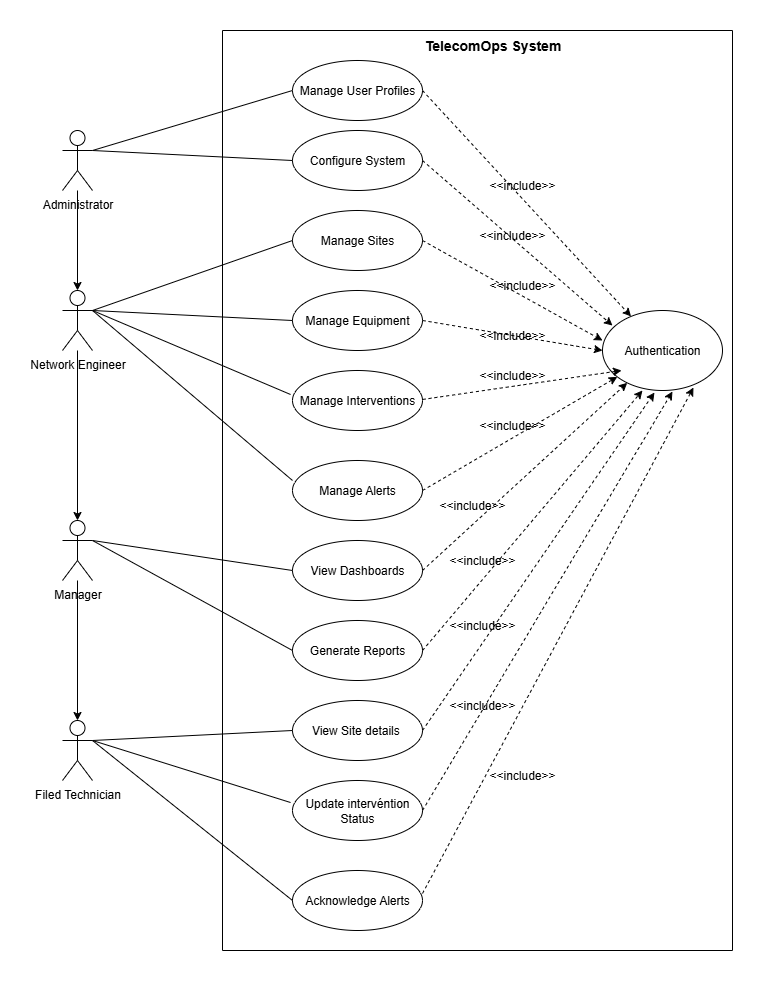
\includegraphics[width=0.95\linewidth]{img/chap_02/TelecomOps_UseCase_Diagram.png}
    \caption{Global Use Case Diagram}
    \label{fig:use_case_global}
\end{figure}
\vspace{1cm}

\section{System Architecture}
In this section, we describe the complete system architecture of the TelecomOps application, including the technological stack, component interactions, and deployment strategy.

\subsection{Architecture Overview}
The TelecomOps system follows a modern three-tier architecture built with Next.js for the frontend and Supabase for backend services. The architecture ensures clear separation of concerns, scalability, and maintainability. The main components include the presentation layer (Next.js), application layer (Supabase), and data layer (PostgreSQL).

\begin{figure}[hbt!]
    \centering
    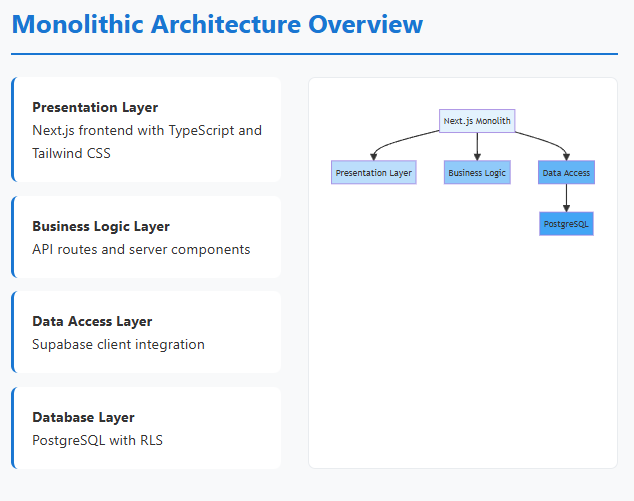
\includegraphics[width=0.9\linewidth]{img/chap_02/architecture_overview.png}
    \caption{Three-Tier Architecture Overview}
    \label{fig:architecture_overview}
\end{figure}

\subsection{Technology Stack}
The application utilizes a modern technology stack that ensures performance, scalability, and developer productivity:

\begin{itemize}
\item \textbf{Frontend:} Next.js 14 with TypeScript and Tailwind CSS
\item \textbf{Backend:} Supabase (PostgreSQL, Authentication, Real-time)
\item \textbf{Deployment:} Vercel (Frontend) and Supabase Cloud (Backend)
\item \textbf{Database:} PostgreSQL with Row Level Security
\end{itemize}

\begin{figure}[hbt!]
    \centering
    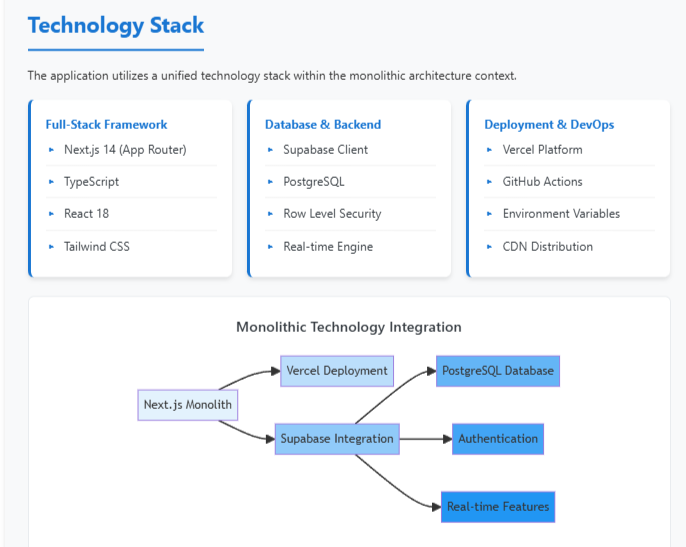
\includegraphics[width=0.85\linewidth]{img/chap_02/technology_stack.png}
    \caption{Technology Stack Components}
    \label{fig:technology_stack}
\end{figure}

\subsection{Database Architecture}
The database schema is designed to efficiently manage telecommunications site data, equipment, interventions, and alerts. The entity-relationship diagram below illustrates the comprehensive data model.

\begin{figure}[hbt!]
    \centering
    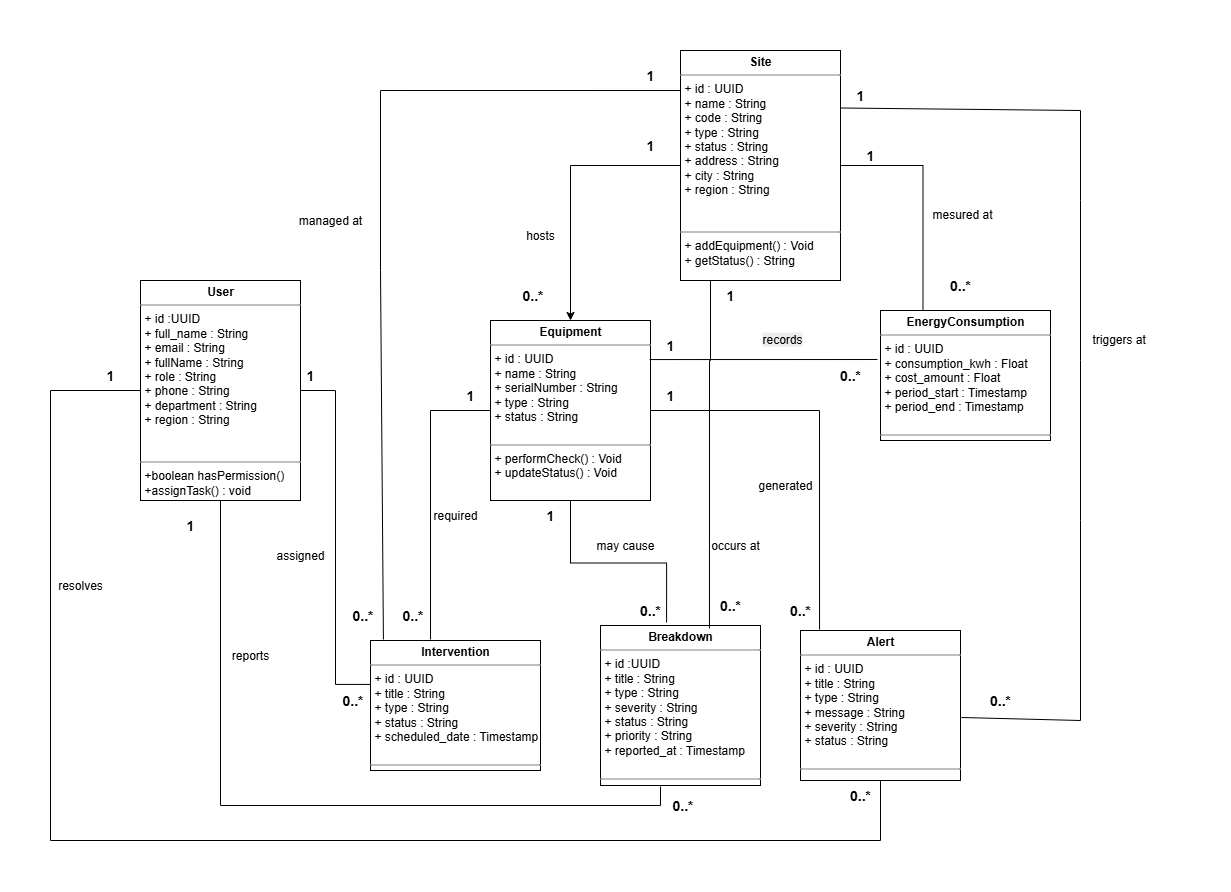
\includegraphics[width=0.95\linewidth]{img/chap_02/database_er_diagram.png}
    \caption{Database Entity-Relationship Diagram}
    \label{fig:database_er_diagram}
\end{figure}

\subsection{Data Flow Architecture}
The system follows a structured data flow pattern where user interactions are processed through multiple layers, ensuring security and data consistency at each step.

\begin{figure}[hbt!]
    \centering
    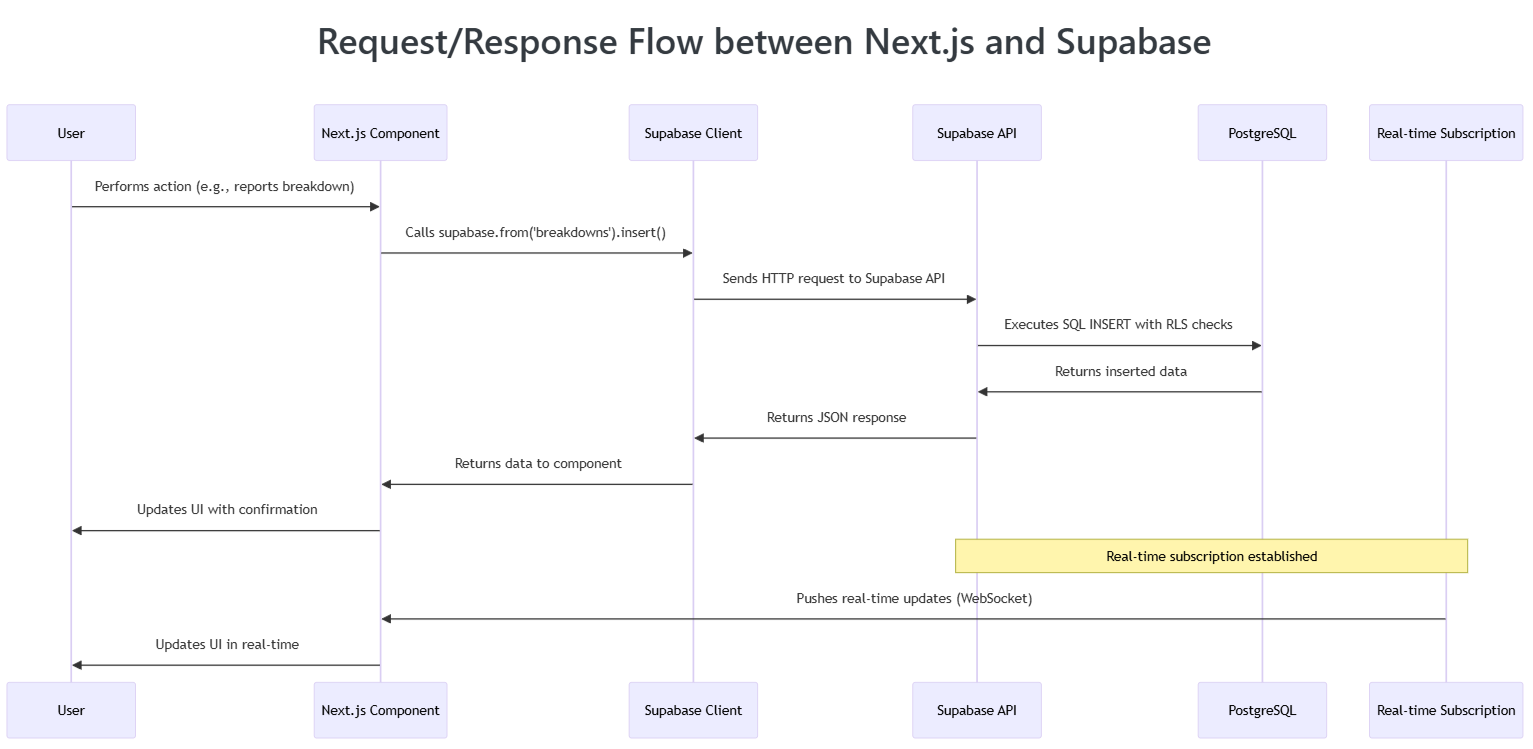
\includegraphics[width=0.9\linewidth]{img/chap_02/data_flow_architecture.png}
    \caption{Data Flow Architecture}
    \label{fig:data_flow_architecture}
\end{figure}

\subsection{Security Architecture}
Security is implemented at multiple layers, including transport security, application-level authentication, and database row-level security policies.

\begin{figure}[hbt!]
    \centering
    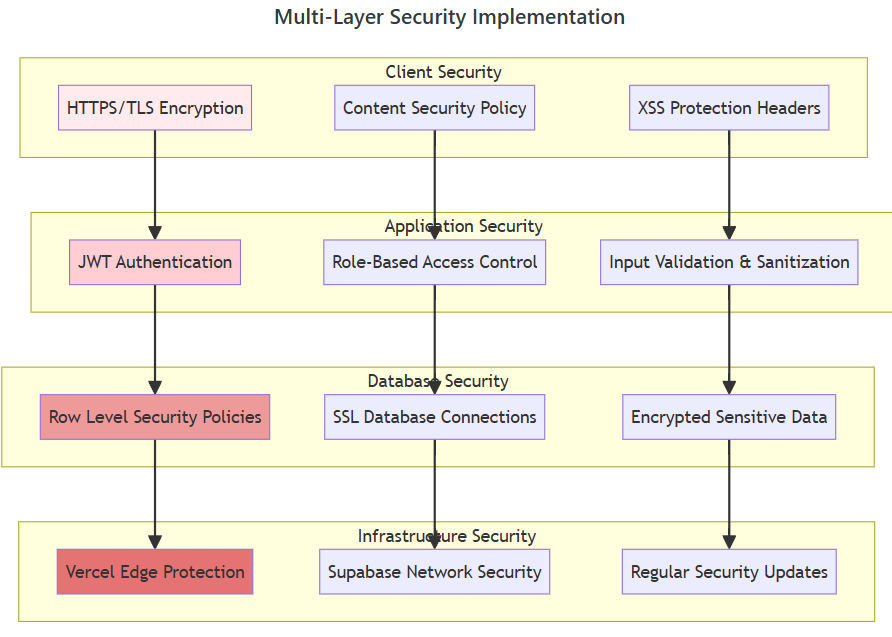
\includegraphics[width=1\linewidth]{img/chap_02/security_architecture.png}
    \caption{Multi-Layer Security Architecture}
    \label{fig:security_architecture}
\end{figure}

\subsection{Deployment Architecture}
The application is deployed using modern cloud platforms that provide scalability, reliability, and global availability.

\begin{figure}[hbt!]
    \centering
    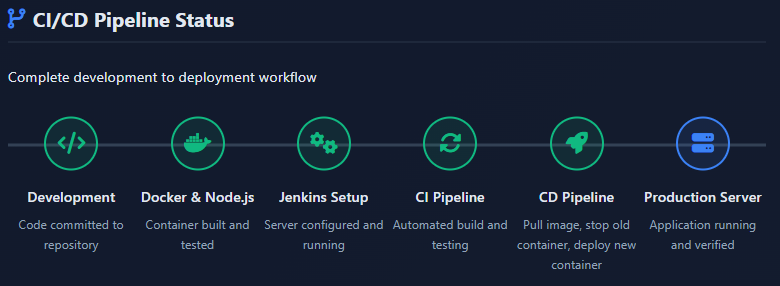
\includegraphics[width=0.85\linewidth]{img/chap_02/deployment_architecture.png}
    \caption{Cloud Deployment Architecture}
    \label{fig:deployment_architecture}
\end{figure}

\subsection{Component Interactions}
The system components interact through well-defined APIs and real-time subscriptions, ensuring efficient communication between the frontend and backend services.

\subsubsection{Next.js Frontend}
The Next.js application handles both server-side rendering and client-side interactions, providing a seamless user experience while maintaining optimal performance.

\subsubsection{Supabase Backend Services}
Supabase provides multiple backend services including:
\begin{itemize}
\item Authentication and authorization management
\item Auto-generated REST APIs from database schema
\item Real-time subscriptions for live data updates
\item File storage and management
\end{itemize}

\subsubsection{PostgreSQL Database}
The PostgreSQL database implements Row Level Security (RLS) policies to ensure data access is strictly controlled based on user roles and permissions.

\subsection{Architecture Benefits}
The chosen architecture provides several significant advantages:

\begin{itemize}
\item \textbf{Scalability:} Cloud-native design allows horizontal scaling
\item \textbf{Maintainability:} Clear separation of concerns simplifies updates
\item \textbf{Security:} Multi-layer security implementation protects sensitive data
\item \textbf{Performance:} Server-side rendering and CDN distribution ensure fast loading
\item \textbf{Real-time Capabilities:} WebSocket connections enable live updates
\end{itemize}

\section{Application Security}
Security is an essential aspect in any web application, especially when it comes to protecting sensitive data and ensuring that only authorized people can access resources. In this project, we have adopted a modern approach to manage user authentication and authorization by integrating Supabase, an open-source Backend-as-a-Service platform.

\subsection{Definition of Supabase}
Supabase is an open-source Backend-as-a-Service platform that provides database, authentication, real-time subscriptions, and API services. It allows centralized management of user identities and access for modern applications.

\subsection{Supabase Security Features}
Supabase ensures unified identity and access management, based on several key features that structure its operation:

\vspace{0.5cm}

\begin{itemize}
\item \textbf{User and Role Management:} \\
Users are created and managed through Supabase authentication system and each user can be assigned to one or more roles. Roles determine user permissions in the application based on their job function (Administrator, Network Engineer, Field Technician, Manager).

\vspace{0.5cm}

\item \textbf{Authentication Process:} \\
When the user attempts to log in, they interact directly with Supabase secure authentication service.
After successful login verification, Supabase generates an access token (JWT) containing user information (name, email, role, permissions) and returns it to the application.

\vspace{0.5cm}

\item \textbf{Authorization Control:} \\
The system verifies the access token received in each request to ensure that the user has the necessary permissions to access the requested resource or perform the requested action.
\end{itemize}

\subsection{Interaction with Application Components}
In a modern architecture, interaction between different systems relies on efficient authentication and authorization management. Here is a detailed overview of the flow and integrations necessary to ensure this communication.

\vspace{0.5cm}

\begin{itemize}
\item \textbf{Frontend Application:} \\
The frontend, developed with Next.js and TypeScript, uses Supabase JavaScript client library to manage user authentication. When a user attempts to access the TelecomOps application, Supabase checks if they are already logged in. If not, the user is redirected to the secure login interface to enter their credentials. Once authenticated, Supabase returns an access token that the frontend stores securely. This token is then included in requests sent to API endpoints, enabling access to secured telecom operations. This flow ensures centralized authentication and secure communication between different parts of the application.

\vspace{0.5cm}

\item \textbf{Backend API System:} \\
The backend, built with Next.js API routes, is configured to validate access tokens generated by Supabase using secure server-side libraries. Each request sent to API endpoints must include a valid token in the HTTP header in the form Authorization: Bearer <token>. When receiving a request, the backend decodes this token to verify the user identity and role-based permissions. Access to different API endpoints (sites management, equipment tracking, interventions, alerts) is then controlled using middleware and Row Level Security policies, ensuring precise authorization control for telecom operations.

\vspace{0.5cm}

\item \textbf{Database Security (PostgreSQL):} \\
Business data, such as site information, equipment details, maintenance interventions, and network alerts, are stored in a PostgreSQL database managed by Supabase. Supabase ensures security through Row Level Security (RLS) policies that guarantee only authorized requests reach the database based on user roles and permissions. Once these requests are validated, they are processed normally on the PostgreSQL database with additional security layers protecting sensitive telecom infrastructure data.
\end{itemize}

\subsection{Global Security Flow}
The global security flow described below illustrates the different stages of secure interaction between systems:

\begin{enumerate}
\item The user attempts to access the TelecomOps application via the web interface.
\item Supabase authenticates the user credentials and generates a secure access token.
\item The frontend sends requests to API endpoints with the access token included.
\item The backend verifies the token with Supabase and authorizes or denies the request based on user roles and permissions.
\item If authorized, the backend executes the telecom operation on PostgreSQL and returns the secure response to the frontend.
\end{enumerate}

\begin{figure}[H]
    \centering
    \includegraphics[width=1\linewidth]{img/architecture/supabase_security_flow.png}
    \caption{Global Security Flow of TelecomOps Authentication}
    \label{fig:security_flow}
\end{figure}

\subsection{Security Benefits}
The Supabase security implementation provides several advantages for the TelecomOps system:

\vspace{0.5cm}

\begin{itemize}
\item \textbf{Centralized Security Management:} \\
All authentication and authorization logic is handled by Supabase, reducing security complexity and potential vulnerabilities.

\vspace{0.5cm}

\item \textbf{Role-Based Access Control:} \\
Different user types (Administrator, Network Engineer, Field Technician, Manager) have appropriate access levels to telecom operations and sensitive network data.

\vspace{0.5cm}

\item \textbf{Data Protection:} \\
Row Level Security policies ensure that users can only access telecom site data and equipment information relevant to their role and assigned responsibilities.

\vspace{0.5cm}

\item \textbf{Secure Communication:} \\
All data transmission between components uses encrypted HTTPS connections with JWT token validation for additional security layers.
\end{itemize}
        \clearpage
        
        
        \chapter*{Conclusion générale}
\addcontentsline{toc}{chapter}{Conclusion générale}
\markboth{\textbf{Conclusion générale}}{}


        \clearpage
        
        % @author: Stoufa
		% the command `\nocite{*}` is mandatory to avoid the “no \citation commands” error
        % https://tex.stackexchange.com/questions/18045/problem-with-compiling-bibtex-no-citation-commands-error
        %\nocite{*}
        
         
\chapter*{Bibliographie}
\addcontentsline{toc}{chapter}{Bibliographie}
\markboth{Bibliographie}{}
\stepcounter{chapter}
\addtocontents{lot}{\vspace{3.8mm}}
\addtocontents{lof}{\vspace{3.8mm}}

[B1]   Pierre Pezziardi, Référentiel des Pratiques Agiles, édition ebook.2013
        \clearpage
        
        \printbibliography[title={Webographie},heading=bibintoc]
        
       
        
        % \chapter*{Annexes}
\addcontentsline{toc}{chapter}{Annexes}
\markboth{Annexes}{}
\stepcounter{chapter}
\addtocontents{lot}{\vspace{3.8mm}}
\addtocontents{lof}{\vspace{3.8mm}}

%Mettez vos annexes ici...

%===================== ANNEXE 1 =====================%

        % \clearpage

    \backmatter
        %===== File containing the back cover of the document =====%
%                                                          %
% Copyright (C) ISI - All Rights Reserved                  %
% Proprietary                                              %
% Written by Med Hossam <med.hossam@gmail.com>, April 2016 %
%                                                          %
% @author: HEDHILI Med Houssemeddine                       %
% @linkedin: http://tn.linkedin.com/in/medhossam           %
%==========================================================%

%== It's advised to not modify the content of this file ===%
% To set your information, go to global_config.tex file    %
%==========================================================%

\thispagestyle{backcover}
\newgeometry{bottom=25mm,left=15mm,top=20mm,right=15mm}

\begin{changemargin}{3mm}{0cm}
    \begin{minipage}[c]{0.96\columnwidth}
        
        
        % {\ifthenelse{\boolean{wantToTypeCompanyAddress}}
        % {% IF TRUE
        %     \vskip5mm
        % }{\vskip8mm}}
        
        \selectlanguage{french}
        
        {\LARGE\textbf{Résumé}}
        \vskip1mm
            \begingroup
                \large
                \@frenchAbstract
            \endgroup
        \vskip1mm
        {\textbf{Mots clés : }
            \begingroup
                \@frenchAbstractKeywords
            \endgroup
        }
        
        {\vskip25mm}
        
        \selectlanguage{english}
        {\LARGE\textbf{Abstract}}
        \vskip1mm
            \begingroup
                \large
                \@englishAbstract
            \endgroup
        \vskip1mm
        {\textbf{Keywords : }
            \begingroup
                \@englishAbstractKeywords
            \endgroup
        }
    \end{minipage}
    
\end{changemargin}
    
\end{document}